\documentclass[a4paper,11pt]{article}
\usepackage[utf8]{inputenc}
\usepackage[italian]{babel}
\usepackage{amsmath, amssymb}
\usepackage{listings}
\usepackage{color}
\usepackage{hyperref}
\usepackage{geometry}
\usepackage{graphicx}
\usepackage{listings}
\usepackage{xcolor}
\usepackage[utf8]{inputenc}

\geometry{a4paper, margin=1in}

% Colors for code listings
\definecolor{commentgray}{gray}{0.5}
\definecolor{stringgreen}{rgb}{0,0.6,0}
\definecolor{keywordblue}{rgb}{0,0,0.6}

% Listing settings for code
\lstset{
    basicstyle=\ttfamily\small,
    keywordstyle=\color{keywordblue},
    stringstyle=\color{stringgreen},
    commentstyle=\color{commentgray}\itshape,
    breaklines=true,
    frame=none,
    numbers=none,
    numberstyle=\tiny,
    tabsize=2,
    showstringspaces=false,
    captionpos=b
}

\title{\textbf{Relazione del Progetto di Programmazione Logica e Funzionale}}
\author{Giaconi Christian, Giacomo Rossi\\Matricola: 314045, 314671}
\date{\today}

\begin{document}

\maketitle

\newpage
\tableofcontents

\newpage
\section{Specifica del problema}
\itshape
Scrivere un programma in Haskell e un programma in Prolog per implementare un sistema di raccomandazione di canzoni. Il sistema suggerisce canzoni a un utente basandosi sulle sue preferenze musicali e utilizza un punteggio di gradimento per ordinare le canzoni più popolari o rilevanti.

\newpage
\section{Analisi del problema}
\subsection{Dati in ingresso}
\begin{itemize}
    \item Un file contenente le canzoni nel formato:
    \begin{verbatim}
    Titolo,Artista,Genere,Punteggio
    \end{verbatim}
    \item Una lista di generi preferiti.
    \item Pesi numerici assegnati ai generi preferiti.
\end{itemize}

\subsection{Dati in uscita}
\begin{itemize}
    \item Una classifica ordinata di canzoni basata sui punteggi ponderati.
    \item Eventuali messaggi di errore o conferma nelle interazioni utente.
\end{itemize}

\subsection{Relazioni tra i dati}
Ogni canzone è caratterizzata da un titolo, un artista, un genere, e un punteggio. Il punteggio ponderato è calcolato come:
\[
Punteggio\ Ponderato = Punteggio \times Peso\_{Genere}
\]
se il genere della canzone appartiene ai generi preferiti, altrimenti è uguale al punteggio originale.

\newpage
\section{Progettazione dell'algoritmo}
\subsection{Scelte di progetto}
Per sviluppare il sistema di raccomandazione musicale, abbiamo adottato approcci distinti per ciascuno dei linguaggi richiesti, Haskell e Prolog, al fine di sfruttare al meglio le peculiarità di ciascuno.

In \textbf{Haskell}, abbiamo deciso di rappresentare le canzoni utilizzando tipi di dati strutturati. Questa scelta ci consente di garantire una gestione chiara e sicura delle informazioni musicali, sfruttando le capacità del sistema di tipi statico per ridurre errori e facilitare l'implementazione delle operazioni. Le canzoni vengono caricate da un file di testo, che deve rispettare un formato predefinito (CSV), per consentire l'integrazione di dataset esterni senza modificare il codice sorgente. La scelta di utilizzare un file di testo è stata motivata dalla necessità di mantenere il sistema flessibile e facilmente adattabile a dataset di dimensioni variabili.

In \textbf{Prolog}, invece, abbiamo optato per una rappresentazione tramite predicati dinamici. Le canzoni sono caricate all’interno del programma attraverso il predicato \texttt{carica\_canzoni/0}, che utilizza \texttt{assertz/1} per definire dinamicamente ogni canzone come un fatto nella base di conoscenza. Questo approccio ci permette di manipolare i dati con la semantica dichiarativa propria di Prolog, evitando problematiche legate all’importazione di file esterni. Ogni canzone è rappresentata da un predicato \texttt{canzone/4}, che descrive il titolo, l’artista, il genere e il punteggio. La struttura dati utilizzata è completamente dinamica, consentendo aggiunte o modifiche in tempo reale senza la necessità di ridefinire l’intero dataset.

\begin{itemize}
    \item \textbf{Haskell:}
    \begin{itemize}
        \item L’uso di file di testo consente di estendere il dataset semplicemente aggiungendo nuove righe al file.
        \item Le funzioni per la manipolazione delle stringhe e la costruzione di tipi di dati strutturati in Haskell rendono questa operazione relativamente semplice e modulare.
        \item Inoltre, Haskell permette un trattamento funzionale dei dati, come la mappatura e il filtraggio, che è particolarmente utile per calcolare e ordinare i punteggi ponderati.
    \end{itemize}
    \item \textbf{Prolog:}
    \begin{itemize}
        \item La rappresentazione tramite predicati è particolarmente adatta per le relazioni tra canzoni, generi e preferenze dell’utente.
        \item Caricare le canzoni come fatti dinamici permette di utilizzare direttamente la logica del linguaggio per effettuare operazioni come il filtraggio e l’ordinamento basato sui punteggi.
        \item Questo approccio evita la necessità di definire una sintassi di input complessa, sfruttando la semplicità dichiarativa propria di Prolog.
    \end{itemize}
    \item \textbf{Gestione dell’input e output:}
    \begin{itemize}
        \item In Haskell, il file di testo richiede un parsing iniziale per costruire una lista di canzoni. Il formato CSV garantisce una struttura standard e compatibile con molti strumenti di editing.
        \item In Prolog, invece, la definizione diretta nel predicato \texttt{carica\_canzoni/0} semplifica l’esecuzione e permette di focalizzarsi sull’elaborazione delle raccomandazioni piuttosto che sulla gestione dell’input.
    \end{itemize}
\end{itemize}

Queste scelte rispecchiano la necessità di bilanciare semplicità implementativa e aderenza ai paradigmi di programmazione dichiarativa e funzionale, garantendo al contempo un'esperienza utente coerente e priva di ambiguità.

\subsection{Passi dell'algoritmo}
I passi principali dell'algoritmo, comuni sia per l'implementazione in Haskell che in Prolog, sono i seguenti:

\begin{enumerate}
    \item \textbf{Caricare le canzoni:} 
    \begin{itemize}
        \item In Haskell, le canzoni vengono caricate da un file di testo in formato CSV, che viene parsato per costruire una lista di canzoni.
        \item In Prolog, le canzoni sono definite all’interno del programma attraverso il predicato \texttt{carica\_canzoni/0}.
    \end{itemize}
    \item \textbf{Inserire le preferenze dell'utente:} 
    L’utente fornisce i generi musicali preferiti e i relativi pesi, che influenzeranno il calcolo dei punteggi ponderati.
    \item \textbf{Calcolare i punteggi ponderati:} 
    Per ogni canzone, viene calcolato un punteggio combinando il peso associato al genere con il punteggio individuale della canzone.
    \item \textbf{Ordinare le canzoni per punteggio ponderato:} 
    Le canzoni vengono ordinate in ordine decrescente rispetto al punteggio ponderato, così da ottenere una classifica delle raccomandazioni.
    \item \textbf{Stampare la classifica:} 
    L’algoritmo produce in output la lista ordinata delle canzoni con i rispettivi punteggi, offrendo una chiara visualizzazione per l’utente.
\end{enumerate}

\newpage
\section{Implementazione dell'algoritmo}
\subsection{Implementazione in Haskell}
Il file \texttt{raccomandazioni.hs} implementa l'algoritmo in Haskell. Un esempio di calcolo dei punteggi ponderati:
\begin{lstlisting}[language=Haskell,caption=raccomandazioni.hs]
    -- #########################################################
    -- # Corso di Programmazione Logica e Funzionale           #
    -- # Progetto di raccomandazione di canzoni                #
    -- # Studente: Giaconi Christian, Giacomo Rossi            #
    -- # Matricola: 314045, 314671                             #
    -- #########################################################
    
    {- Specifica:
        Scrivere un programma in Haskell per implementare un sistema avanzato di raccomandazione di canzoni.
        Il sistema suggerisce canzoni a un utente in base a:
        - Preferenze per uno o più generi musicali specificati.
        - Un sistema di punteggio ponderato per dare priorità a canzoni più rilevanti.
        L'utente deve fornire un file di testo con le canzoni nel seguente formato:
            Titolo,Artista,Genere,Punteggio
        Dove "Punteggio" è un intero da 1 a 10.
        Le canzoni saranno ordinate in base al punteggio ponderato e filtrate per genere.
    -}
    
    module Main where
    
    import Data.List (sortOn, nub, intercalate)
    import Data.Maybe (mapMaybe)
    import Data.Ord (Down(..))
    import qualified Data.Map as Map
    import System.IO.Error(isDoesNotExistError)
    import Control.Exception (catch, IOException)
    import Text.Read (readMaybe)
    
    -- #########################################################
    -- Definizioni dei tipi di dati
    -- #########################################################
    
    -- | La struttura 'Canzone' rappresenta una canzone con:
    -- - titolo: il titolo della canzone.
    -- - artista: l'artista che la interpreta.
    -- - genere: il genere musicale della canzone.
    -- - punteggio: un punteggio assegnato (da 1 a 10).
    data Canzone = Canzone
        { titolo    :: String
        , artista   :: String
        , genere    :: String
        , punteggio :: Int
        } deriving (Show, Eq)
    
    -- | PesiGeneri è una mappa che associa un genere musicale a un peso
    -- che influenza la priorità delle raccomandazioni.
    type PesiGeneri = Map.Map String Double
    
    -- #########################################################
    -- Main: Menu interattivo
    -- #########################################################
    
    -- | Funzione principale che avvia il menu interattivo.
    main :: IO ()
    main = menuLoop Nothing Map.empty
    
    -- | Gestisce il menu principale, mantenendo lo stato del sistema:
    -- - maybeCanzoni: un elenco opzionale delle canzoni caricate.
    -- - pesi: i pesi dei generi preferiti, gestiti dall'utente.
    menuLoop :: Maybe [Canzone] -> PesiGeneri -> IO ()
    menuLoop maybeCanzoni pesi = do
        putStrLn "\n--- Sistema di Raccomandazione Musicale ---"
        putStrLn "1. Carica un file con le canzoni"
        putStrLn "2. Gestisci i generi preferiti (aggiungi o modifica)"
        putStrLn "3. Stampa la classifica delle canzoni"
        putStrLn "4. Stampa i generi preferiti con il relativo punteggio"
        putStrLn "5. Esci"
        putStrLn "Seleziona un'opzione:"
        scelta <- getLine
        case scelta of
            "1" -> caricaCanzoni >>= (`menuLoop` pesi) . Just
            "2" -> selezionaGeneriPreferitiEImpostaPesi maybeCanzoni pesi >>= menuLoop maybeCanzoni
            "3" -> raccomandaCanzoni maybeCanzoni pesi >> menuLoop maybeCanzoni pesi
            "4" -> visualizzaGeneriPreferiti pesi >> menuLoop maybeCanzoni pesi
            "5" -> putStrLn "Grazie per aver usato il sistema di raccomandazione. Arrivederci!"
            _   -> putStrLn "Opzione non valida. Riprova." >> menuLoop maybeCanzoni pesi
    
    -- #########################################################
    -- Funzioni di caricamento e gestione dei dati
    -- #########################################################
    
    -- | Carica un file di testo, legge i dati delle canzoni e li
    -- trasforma in una lista di Canzone.
    -- Il file deve avere un formato valido: Titolo,Artista,Genere,Punteggio.
    caricaCanzoni :: IO [Canzone]
    caricaCanzoni = do
        nomeFile <- chiediNomeFile
        contenuto <- readFile nomeFile
        let canzoni = mapMaybe analizzaCanzone (lines contenuto)
        if null canzoni
            then putStrLn "Errore: il file non contiene dati validi! Riprova." >> caricaCanzoni
            else putStrLn "File caricato con successo!" >> return canzoni
    
    -- | Richiede all'utente di inserire il nome del file con le canzoni
    -- e ne effettua una validazione dell'input tramite la funzione validaFile.
    chiediNomeFile :: IO FilePath
    chiediNomeFile = do
        putStrLn "Inserire il nome del file:"
        nomeFile <- getLine
        esito_lettura <- validaFile nomeFile
        case esito_lettura of
            Right () -> return nomeFile  -- Restituisce il nome del file se valido
            Left err -> do
                putStrLn $ "Errore: " ++ err
                chiediNomeFile
    
    -- | Controlla se il nome del file è espresso
    -- correttamente e se tale file esiste.
    validaFile :: FilePath -> IO (Either String ())
    validaFile nomeFile =
        catch (readFile nomeFile >> return (Right ()))
              (\e -> if isDoesNotExistError e
                     then return $ Left "File non trovato!"
                     else return $ Left "Errore durante l'apertura del file.")
    
    -- | Permette all'utente di scegliere
    -- i generi preferiti e assegnare un peso a ciascuno di essi.
    selezionaGeneriPreferitiEImpostaPesi :: Maybe [Canzone] -> PesiGeneri -> IO PesiGeneri
    selezionaGeneriPreferitiEImpostaPesi Nothing pesi = do
        putStrLn "Errore: nessun file caricato. Carica un file prima di continuare."
        return pesi
    selezionaGeneriPreferitiEImpostaPesi (Just canzoni) pesi = do
        let generiDisponibili = nub $ map genere canzoni
        putStrLn $ "Generi disponibili: " ++ intercalate ", " generiDisponibili
        generiSelezionati <- raccogliGeneri generiDisponibili
        aggiornaPesi generiSelezionati pesi
    
    -- | Consente all'utente di inserire i generi
    -- preferiti uno alla volta, terminando con "fine".
    raccogliGeneri :: [String] -> IO [String]
    raccogliGeneri generiDisponibili = do
        putStrLn "Inserisci i generi preferiti uno alla volta. Scrivi 'fine' per terminare."
        loop []
      where
        loop acc = do
            putStrLn "Inserisci un genere preferito:"
            input <- getLine
            if input == "fine"
                then return (nub acc)
                else if input `elem` generiDisponibili
                     then putStrLn ("Genere '" ++ input ++ "' aggiunto ai preferiti.") >> loop (input : acc)
                     else putStrLn "Genere non valido. Riprova." >> loop acc
    
    -- | Consente all'utente di modificare i pesi dei generi preferiti.
    -- Se il genere ha già un peso, l'utente può scegliere di mantenerlo o aggiornarlo.
    aggiornaPesi :: [String] -> PesiGeneri -> IO PesiGeneri
    aggiornaPesi [] pesi = return pesi
    aggiornaPesi (g:gs) pesi = do
        let pesoCorrente = Map.findWithDefault 1.0 g pesi
        putStrLn $ "Peso corrente per il genere '" ++ g ++ "': " ++ show pesoCorrente
        putStrLn "Vuoi aggiornare il peso? (s/n)"
        risposta <- getLine
        if risposta == "s"
            then do
                putStrLn $ "Inserisci il nuovo peso per il genere '" ++ g ++ "':"
                nuovoPeso <- leggiPesoValido
                aggiornaPesi gs (Map.insert g nuovoPeso pesi)
            else do
                putStrLn $ "Peso per il genere '" ++ g ++ "' invariato."
                aggiornaPesi gs pesi
    
    -- #########################################################
    -- Raccomandazioni
    -- #########################################################
    
    -- | Genera e stampa una lista di canzoni consigliate
    -- basandosi sui pesi dei generi e sui punteggi delle canzoni.
    raccomandaCanzoni :: Maybe [Canzone] -> PesiGeneri -> IO ()
    raccomandaCanzoni Nothing _ = putStrLn "Errore: nessun file caricato. Carica un file prima di continuare."
    raccomandaCanzoni (Just canzoni) pesi = do
        let raccomandate = raccomanda pesi canzoni
        if null raccomandate
            then putStrLn "Nessuna canzone trovata con i pesi attuali."
            else stampaClassifica raccomandate
    
    -- #########################################################
    -- Funzioni ausiliarie
    -- #########################################################
    
    -- | Converte una riga di testo in un oggetto Canzone.
    -- Restituisce Nothing se la riga non è formattata correttamente.
    analizzaCanzone :: String -> Maybe Canzone
    analizzaCanzone riga =
        case separaTaglia ',' riga of
            [titolo, artista, genere, punteggioStr]
                | "" `notElem` [titolo, artista, genere, punteggioStr]  -- Controlla che tutte le parti siano non vuote
                , Just punteggio <- readMaybe punteggioStr  -- Prova a leggere il punteggio
                , punteggio >= 1 && punteggio <= 10 -> Just (Canzone titolo artista genere punteggio)  -- Verifica che il punteggio sia valido
            _ -> Nothing  -- Restituisce Nothing se la riga non è valida
    
    -- | Divide una stringa in una lista di stringhe, usando un delimitatore.
    separa :: Char -> String -> [String]
    separa _ "" = []
    separa delimiter string =
        let (primo, resto) = break (== delimiter) string
        in primo : case resto of
            [] -> []
            x -> separa delimiter (dropWhile (== delimiter) (tail x))
    
    -- | Divide una stringa in campi separati, pulendo gli spazi.
    separaTaglia :: Char -> String -> [String]
    separaTaglia delimiter string = map (filter (/= ' ')) (separa delimiter string)
    
    -- | Legge un valore di peso valido inserito dall'utente.
    leggiPesoValido :: IO Double
    leggiPesoValido = do
        input <- getLine
        case readMaybe input of
            Just peso | peso > 0 -> return peso
            _ -> putStrLn "Peso non valido. Riprova." >> leggiPesoValido
    
    -- | Calcola il punteggio ponderato per ogni canzone e le ordina.
    raccomanda :: PesiGeneri -> [Canzone] -> [(Double, Canzone)]
    raccomanda pesi canzoni =
        let arricchite = arricchisci pesi canzoni
        in sortOn (Down . fst) arricchite
    
    -- | Calcola il punteggio ponderato per ogni canzone.
    arricchisci :: PesiGeneri -> [Canzone] -> [(Double, Canzone)]
    arricchisci pesi canzoni =
        [ (fromIntegral (punteggio c) * Map.findWithDefault 1.0 (genere c) pesi, c) | c <- canzoni ]
    
    -- | Stampa le canzoni ordinate con il loro punteggio ponderato.
    stampaClassifica :: [(Double, Canzone)] -> IO ()
    stampaClassifica raccomandate =
        mapM_ stampaConPosizione (zip [1..] raccomandate)
        where
            stampaConPosizione (pos, (punteggioPonderato, Canzone titolo artista genere _)) = do
                putStrLn $ "#" ++ show pos ++ " - " ++ titolo
                putStrLn $ "   Artista: " ++ artista
                putStrLn $ "   Genere: " ++ genere
                putStrLn $ "   Punteggio ponderato: " ++ show punteggioPonderato
                putStrLn "-------------------------------------------"
    
    -- | Visualizza i generi preferiti e i pesi associati.
    visualizzaGeneriPreferiti :: PesiGeneri -> IO ()
    visualizzaGeneriPreferiti pesi
        | Map.null pesi = putStrLn "Nessun genere ancora definito."
        | otherwise = do
            putStrLn "I tuoi generi preferiti e pesi associati sono:"
            mapM_ stampaGenere (Map.toList pesi)
    
    -- | Stampa il genere, concatenato al peso suo relativo
    stampaGenere :: (String, Double) -> IO ()
    stampaGenere (genere, peso) = putStrLn $ genere ++ ": " ++ show peso
\end{lstlisting}

\subsection{Implementazione in Prolog}
Il file \texttt{raccomandazioni.pl} implementa l'algoritmo in Prolog. Esempio di ordinamento delle canzoni:
\begin{lstlisting}[language=Prolog,caption=raccomandazioni.pl]
classifica_ordinata(Ordinata) :-
    findall(Punteggio-Titolo, punteggio_ponderato(Titolo, Punteggio), Punteggi),
    sort(1, @>=, Punteggi, Ordinata).
\end{lstlisting}

\newpage
\section{Testing}
\subsection{Testing del programma in Haskell}
\begin{center}
    \textbf{Test 1}
    \par
    \vspace{0.5cm}
    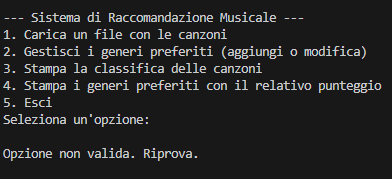
\includegraphics[width=0.5\textwidth]{htest1}
\end{center}
\begin{center}
    \textbf{Test 2}
    \par
    \vspace{0.5cm}
    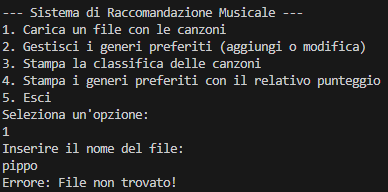
\includegraphics[width=0.5\textwidth]{htest2}
\end{center}
\begin{center}
    \textbf{Test 3}
    \par
    \vspace{0.5cm}
    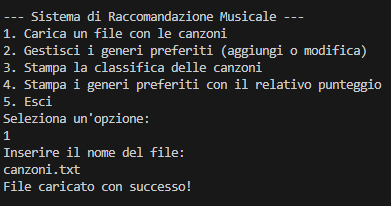
\includegraphics[width=0.5\textwidth]{htest3}
\end{center}

\newpage
\begin{center}
    \textbf{Test 4}
    \par
    \vspace{0.5cm}
    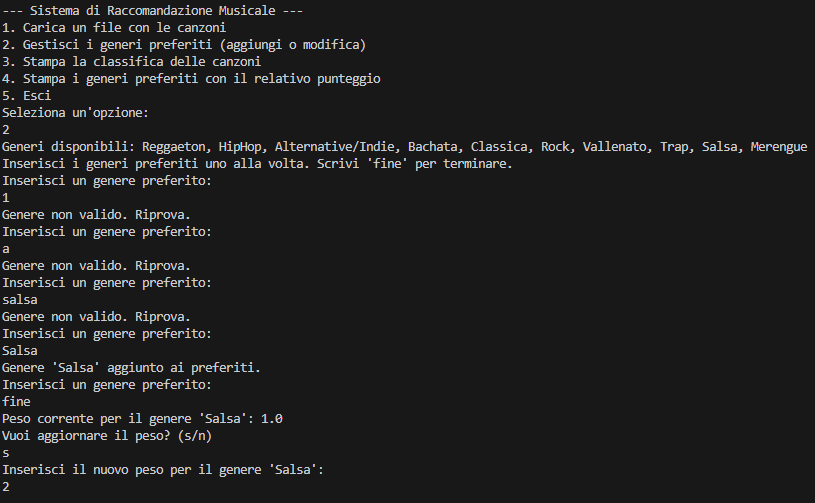
\includegraphics[width=0.5\textwidth]{htest4}
\end{center}
\begin{center}
    \textbf{Test 5}
    \par
    \vspace{0.5cm}
    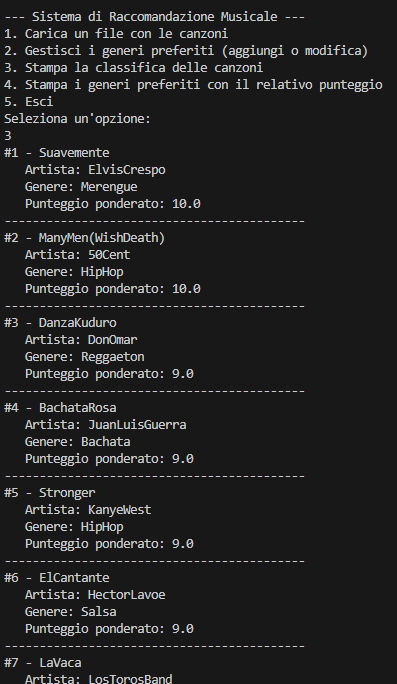
\includegraphics[width=0.5\textwidth]{htest5}
    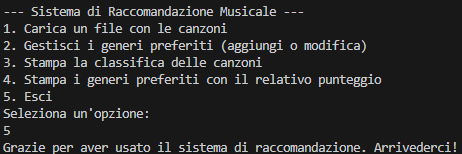
\includegraphics[width=0.5\textwidth]{htest10}
\end{center}

\newpage
\begin{center}
    \textbf{Test 6}
    \par
    \vspace{0.5cm}
    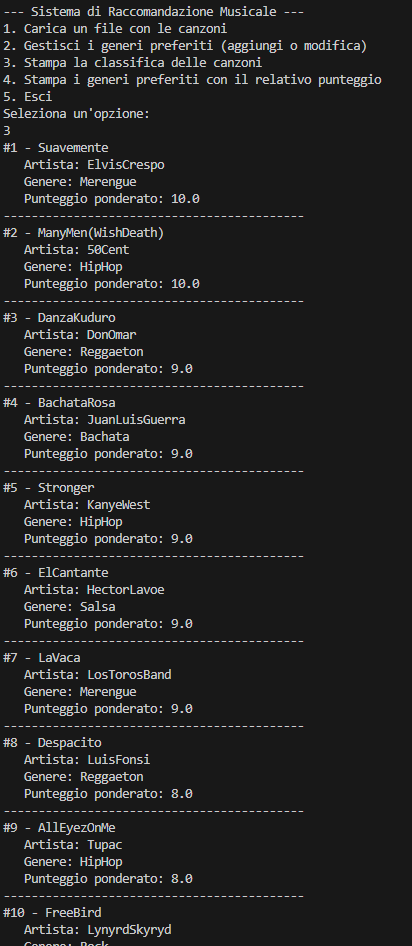
\includegraphics[width=0.5\textwidth]{htest6}
\end{center}

\newpage
\begin{center}
    \textbf{Test 7}
    \par
    \vspace{0.5cm}
    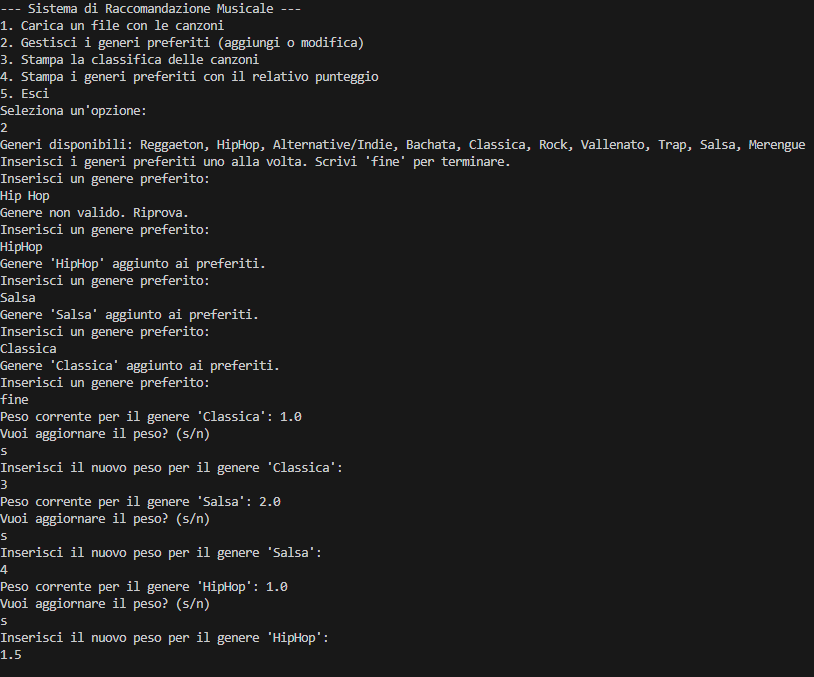
\includegraphics[width=0.5\textwidth]{htest7}
\end{center}
\begin{center}
    \textbf{Test 8}
    \par
    \vspace{0.5cm}
    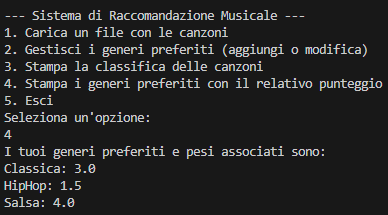
\includegraphics[width=0.5\textwidth]{htest8}
\end{center}

\newpage
\begin{center}
    \textbf{Test 9}
    \par
    \vspace{0.5cm}
    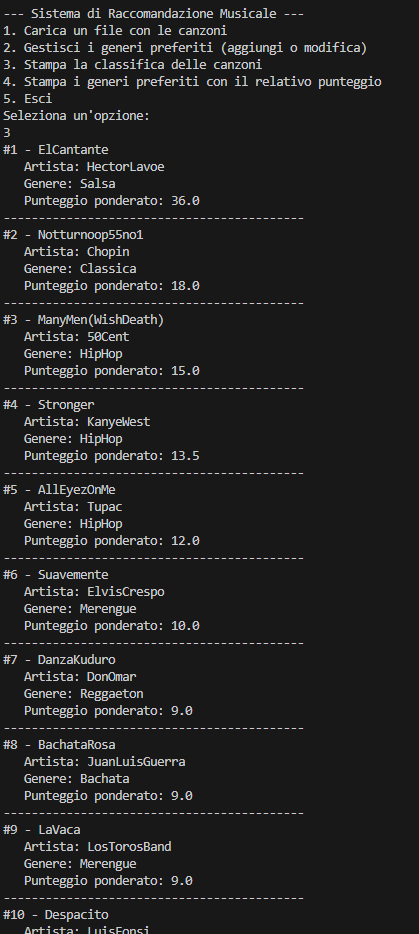
\includegraphics[width=0.5\textwidth]{htest9}
\end{center}
\begin{center}
    \textbf{Test 10}
    \par
    \vspace{0.5cm}
    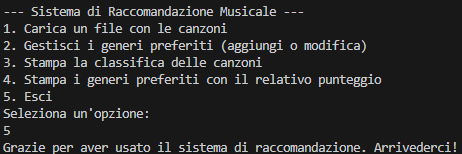
\includegraphics[width=0.5\textwidth]{htest10}
\end{center}
\vspace{1cm}

\newpage
\subsection{Testing del programma in Prolog}

\end{document}
